%% Chapter 5: System design
\chapter{System Design}
\label{chapter:system-design}

\graphicspath{ {report/C5 System Design/assets/} } 

\section{Design of the SSVEP Stimuli}

Naturally, an important part of the SSVEP-based BCI system is the SSVEP stimuli which will be presented to individuals participating in the exhibition (or in general, anyone interacting with the system thereafter). Taking into account design parameters such as stimulus colour, position and contrast mentioned in the literature cited in Section \ref{subsection:evoking-measuring-ssveps}, a basic user interface (UI) was designed with a series of flashing squares as depicted in Figure \ref{fig:ssvep-squares-c5}. This UI was implemented as a lightweight HTML page with basic CSS styling and Javascript to handle animation (flickering of the squares). This decision was made to allow for the simplest and most convenient deployment across any device capable of displaying a web page (mobile or otherwise). The number of blocks being displayed and their labels are subject to adjustment in accordance with other elements of the demonstration beyond the scope of this project.

\begin{figure}][!htb]
    \centering
    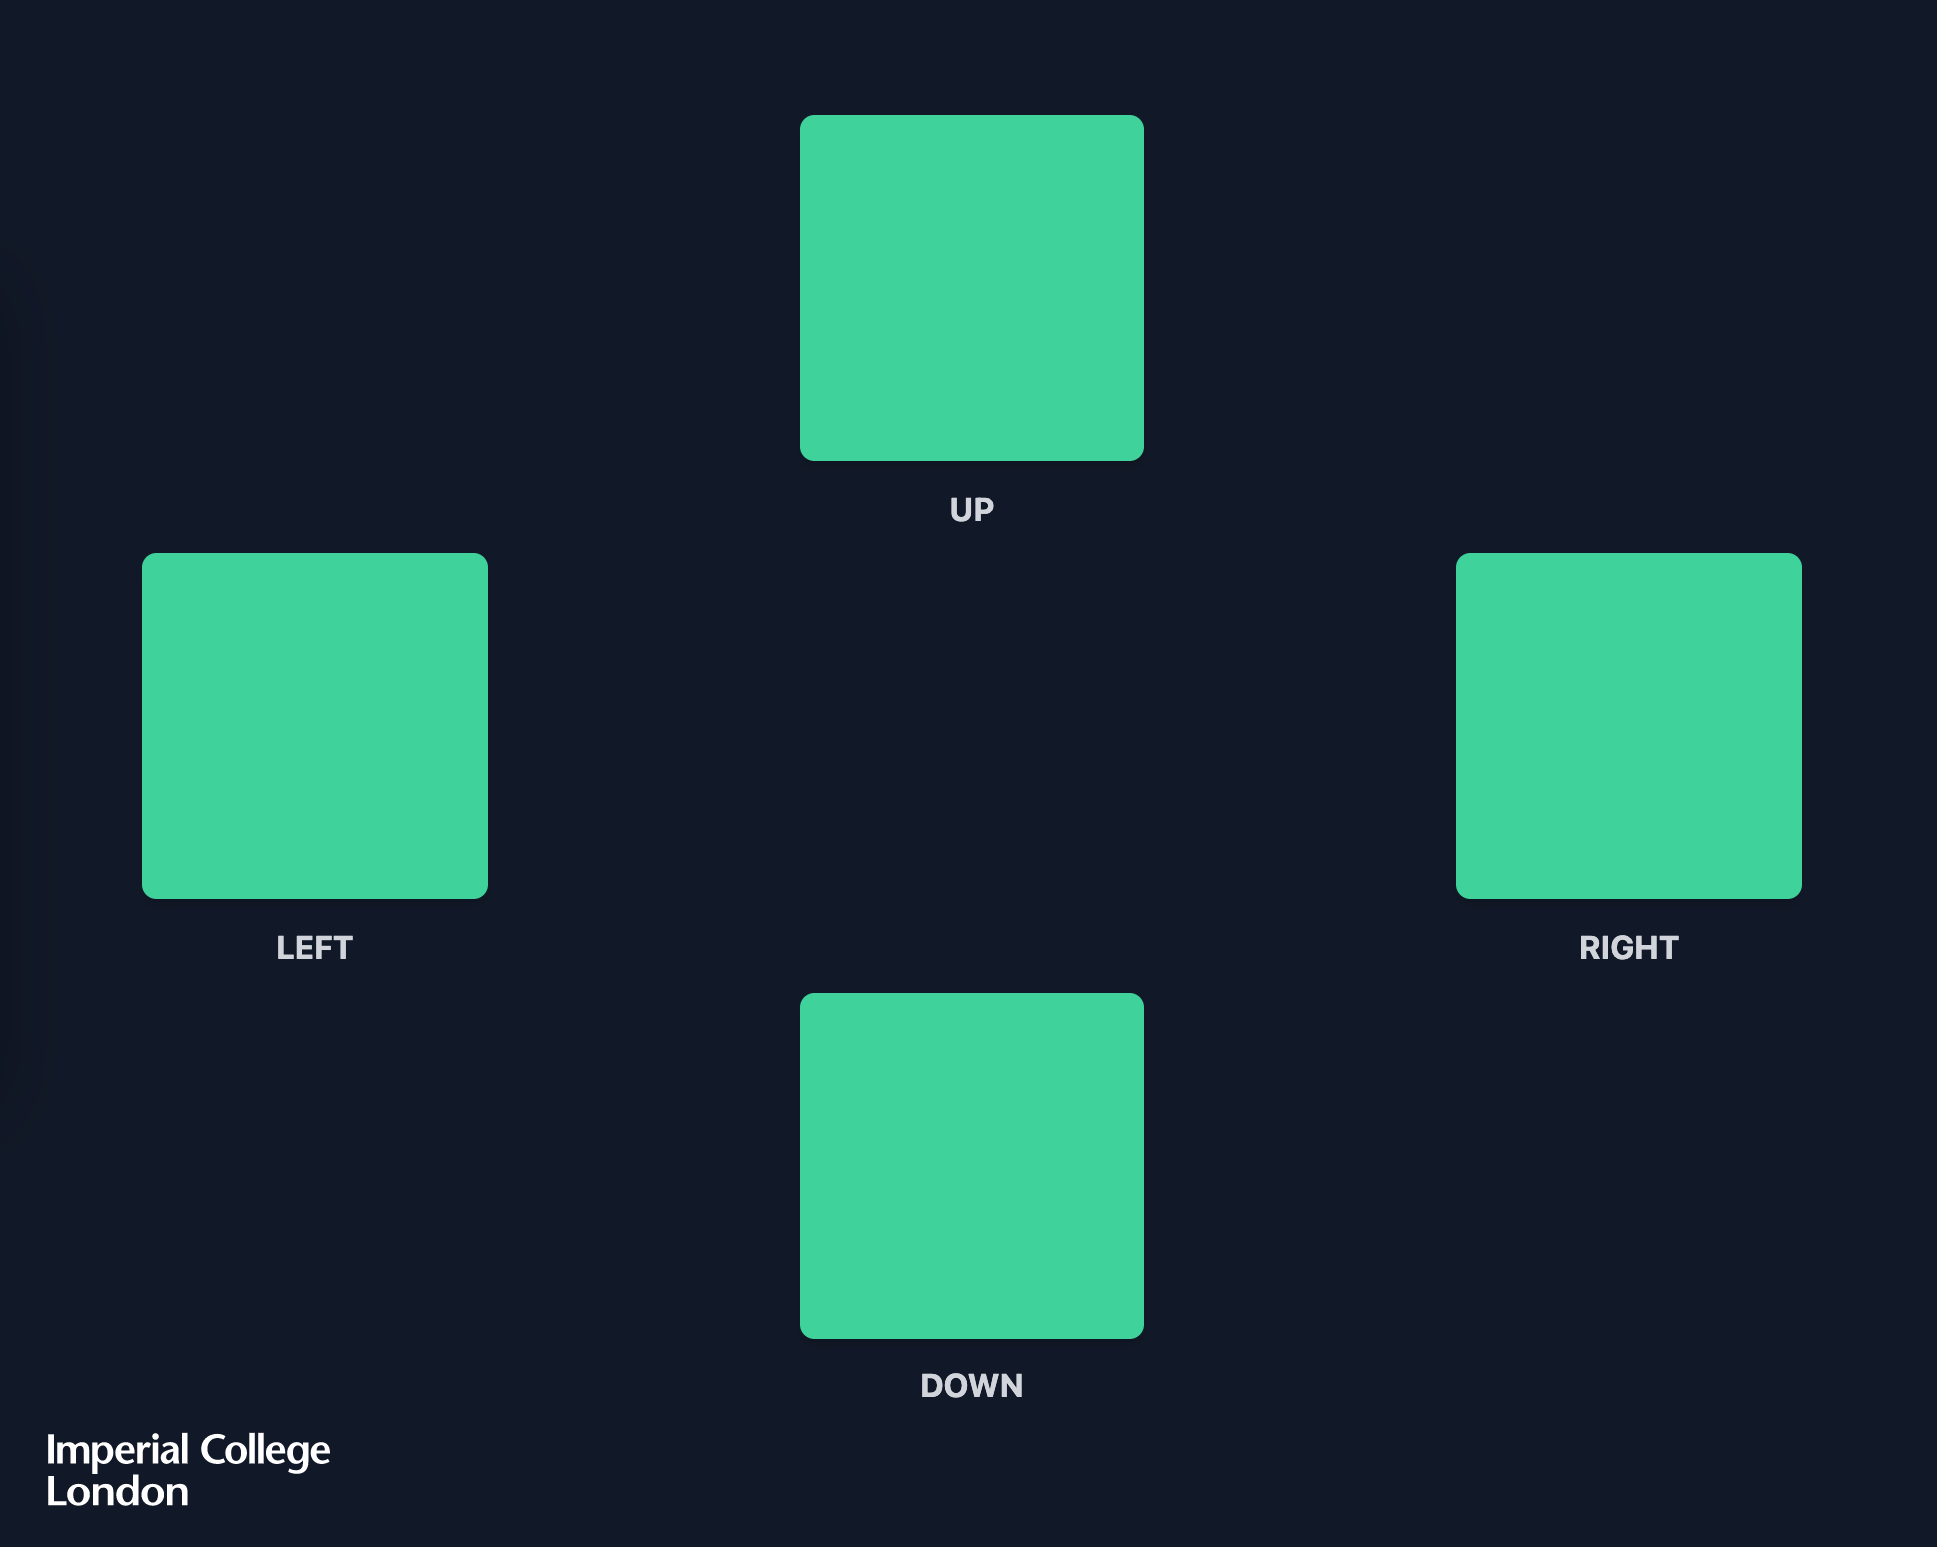
\includegraphics[width=0.8\textwidth]{ssvep-squares}
    \caption{Screen capture of the user interface for displaying SSVEP stimuli. The blocks can be independently set to any flicker frequency of interest.}
    \label{fig:ssvep-squares-c5}
\end{figure}

A key consideration in the design of the SSVEP stimuli is the stimulus frequencies $f_1, \dots, f_n$ to use. As mentioned in Section \ref{subsection:time-frequency-considerations-c2}, similar studies typically use stimulus frequencies between 6Hz and 15Hz for this task. Based on frequencies most commonly selected, the set of stimulus frequencies $\mathcal{F}$ selected for this project were: $\mathcal{F} = \{f_1, \dots, f_n\} = \{7, 8, 10, 12\}$ (all in Hz). Note that, external factors related to this project may only require some subset of $\mathcal{F}$: for example, the stimulus square corresponding to `down' may be omitted if only the other three actions are required in the game or simulation. 

\section{Digital Signal Processing System}

A crucial part in the design of the BCI system is the digital signal processing (DSP) system. The key functions of this system are to digitise, filter and resample the analogue output of the analogue signal processing system presented in Figure \ref{fig:analogue-system-c4}. An overview of the DSP system is shown in Figure \ref{fig:digital-system-c5}.

\begin{figure}
    \centering
    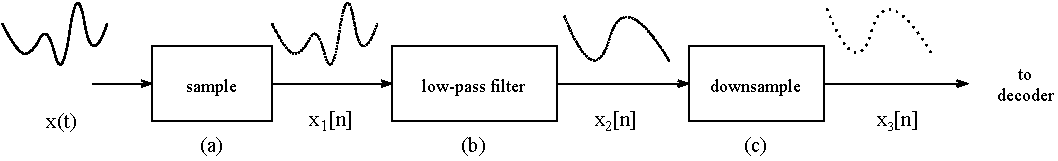
\includegraphics[width=\textwidth]{digital-system}
    \caption{Digital signal processing system}
    \label{fig:digital-system-c5}
\end{figure}

Details of the components shown in Figure \ref{fig:digital-system-c5} are provided below. 

\subsubsection{Sampling}
The analogue signal $x(t)$ digitised to $x_1[n]$ using the 12-bit SAR ADC on-board the ESP32. A sampling frequency of $f_s=256$Hz was selected based for several reasons. First, this is a typical value mentioned in the literature as noted in Section \ref{subsection:time-frequency-considerations-c2}. Second, and more importantly, considering the SSVEP target frequency band 

\subsubsection{Digital low-pass filtering}

\subsubsection{Downsampling}


\begin{enumerate}[label=(\alph*)] % (a), (b), (c), ...
\item sampling
\begin{itemize}
   
\end{itemize}
\item low-pass filter
\begin{itemize}
    \item low-pass filter to isolate the frequency band of interest from DC to $28$Hz. Used to provide greater 50Hz noise rejection to allow for downsampling. 
    \item corner frequency $f_c=32$Hz
    \item $10^{\textrm{th}}$ order elliptical filter
    \item 50Hz rejection characteristics: minimum 17dB, nominal 35dB and maximum 55dB.
\end{itemize}

\item adjustable-gain output amplifier
\begin{itemize}
    \item adjustable gain between 1.745 and 19.2
    \item input low-pass filter dynamics: corner frequency of $f_c=36.35$Hz 
\end{itemize}
\end{enumerate}

\section{Firmware structure}
Discuss Micropython and uLab here, including their features, benefits and potential drawbacks compared to more conventional C/C++.
Discuss module structure and give a diagram of how modules are arranged and what functionality they provide

\subsection{Networking}
Discuss AWS IoT interface and real-time streaming capabilities using MQTT



\section{Algorithm Implementation}



Discuss numerical challenges, precision issues, memory constraints
Discuss some of the auxiliary computational approaches used such as eigenvalue solvers etc

